\documentclass[11pt]{amsart}
\usepackage{amsmath,amsfonts,amssymb,amsthm,verbatim,multirow,url,subfig,footnote,graphicx,array,xr,booktabs,placeins,float}
\usepackage[usenames,dvipsnames]{color}
\usepackage[style=numeric,
doi=false,
isbn=false,
url=false]{biblatex}
\usepackage[utf8]{inputenc}
\usepackage[T1]{fontenc}


\theoremstyle{plain}
\newtheorem{lema}{Lemma}
\newtheorem{coro}{Corollary}
\newtheorem{teo}{Theorem}
\newtheorem{prop}{Proposition}
\theoremstyle{definition}
\newtheorem{ap}{Assumption}
\newtheorem{defin}{Definition}
\theoremstyle{remark}
\newtheorem*{rk}{Remark}
\newcommand{\nn}{\mathbf}
\newcommand{\nns}{\boldsymbol}
\newcommand{\Hcal}{\mathcal H}

\newcommand{\fv}[1]{\color{ForestGreen}\textbf{[FV: #1]}\normalcolor}
\newcommand{\lb}[1]{\color{MidnightBlue}\textbf{[LB: #1]}\normalcolor}

\addbibresource{biblioteca.bib}

\begin{document}
\title[Paleoclimate Reconstruction using INLA.]{Paleoclimate
  Reconstruction and Forecasting of the Northern Hemisphere Temperature using INLA algorithm.}

\author{Luis A. Barboza}
\address{Centro de Investigacion en Matematica Pura y Aplicada (CIMPA), Universidad de Costa Rica\\
San Jos\'e, Costa Rica}
\email{luisalberto.barboza@ucr.ac.cr}


\author{Julien Emile-Geay}
\address{Department of Earth Sciences \\
  University of Southern California \\
  Los Angeles, California, USA.
}
\email{julieneg@usc.edu}

\author{Bo Li}
\address{Department of Statistics \\
  University of Illinois at Urbana-Champaign \\
  Champaign, Illinois, USA.
}
\email{libo@illinois.edu}

\date{\today}
%\date{December 20, 2014}
\keywords{INLA,Paleoclimate Reconstruction,Hierarchical Bayesian Model}
\subjclass[2010]{}
\maketitle

\begin{abstract}
A Paleolimate Reconstruction on the Common Era (1-2000AD) was performed using a
Hierarchical Bayesian Model from three sources of data: proxy data from PAGES2k
project dataset, HadCRUT4 temperature data from the Climatic Research Unit
at the University of East Anglia and external forcing data from several sources.
Instead of using the MCMC approach to solve for the latent variable, we used the
INLA algorithm that shows a similar approximation than previous studies. The use
of external forcings was tested by replace them with a fixed number of
BSplines in the latent equation. Classical goodness-of-fit measures show that there is not a significant
difference between the predictive ability of both approaches. We also employed
the models to forecast the temperature anomalies during the period 2001-2014.
\end{abstract}

\section{Introduction.}
\label{sec:intro}

\section{Integrated Nested Laplace Approximation (INLA).}
\label{sec:inla}

The INLA approach uses a general specification where the mean of a sequence of
observations is a function of the linear structure:
\begin{align*}
  \eta_i = \alpha +\sum_{m-=1}^M\beta_mx_{mi}+\sum_{l=1}^Lf_l(z_{li})
\end{align*}
where $\alpha$ represents an intercept; the coefficients
$\mathbf{\beta} = (\beta_1,\ldots,\beta_M)$ are related to $M$ covariates
$(x_1,\ldots,x_M)$ and $f = \{f_1(\cdot),\ldots,f_L(\cdot)\}$ is a collection of
random effects defined on a set of $L$ covariates $(z_1,\ldots,z_L)$ (see
\cite{Rue2009} and \cite{Blangiardo2013}). Denote the set of random parameters as
$\theta = (\alpha,\beta,f)$ with $K$ hyperparameters $\psi =
\{\psi_1,\ldots,\psi_K\}$. If $y=(y_1,\ldots,y_n)$ denotes the observations, we
can assume conditional independence in the following way:
\begin{align*}
  p(y|\theta,\psi)=\prod_{i=1}^np(y_i|\theta_i,\psi),
\end{align*}
The INLA approach assumes that (1) the vector $\theta$ is multivariate normal with
some precision matrix depending on the hyperparameters $\psi$, and (2) this vector
$\theta$ is conditionally independent given the hyperparameters. These two
assumptions specifies $\theta$ as a Gaussian Markov random field.

The main objectives of the bayesian estimation in this case are to compute the
marginal posterior distribution of each parameter in $\theta$:
\begin{align*}
  p(\theta_i|y) = \int p(\theta_i,\psi|y)d \psi = \int p(\theta_i|\psi,y)p(\psi|y)d \psi
\end{align*}
and the marginal posterior distribution of each hyperparameter:
\begin{align*}
  p(\psi_k|y)=\int p(\psi|y) d\psi_{-k}.
\end{align*}
In order to compute the above, we need to approximate the components $p(\psi|y)$
and $p(\theta_i|\psi,y)$. The first component can be approximated using a
Laplace Approximation (see \cite{Tierney1986}):
\begin{align*}
  p(\psi|y)&=\frac{p(\theta,\psi|y)}{p(\theta|\psi,y)}\propto \frac{p(\psi)p(\theta|\psi)p(y|\theta)}{p(\theta|\psi,y)}\\
           & \approx  \frac{p(\psi)p(\theta|\psi)p(y|\theta)}{\tilde p(\theta|\psi,y)} \Biggm |_{\theta=\theta^*(\psi)} := \tilde p(\psi|y)
\end{align*}
where $\tilde p(\theta|\psi,y)$ is the Gaussian approximation of
$p(\theta|\psi,y)$ and $\theta^*(\psi)$ is its mode (see \cite{Rue2009}). The
second component can be approximated in a similar way:
\begin{align}\label{eq:second}
  p(\theta_i|\psi,y)&=\frac{p((\theta_i,\theta_{-i})|\psi,y)}{p(\theta_{-i}|\theta_i,\psi,y)} \notag \\
  &\approx \frac{p((\theta_i,\theta_{-i})|\psi,y)}{\tilde p(\theta_{-i}|\theta_i,\psi,y)} \Biggm |_{\theta_{-i}=\theta_{-i}^*(\theta_i,\psi)}:=\tilde p(\theta_i|\psi,y)
\end{align}
and $\tilde p(\theta_{-i}|\theta_i,\psi,y)$ is the gaussian approximation of
$p(\theta_{-i}|\theta_i,\psi,y)$. In this case $\theta=(\theta_i,\theta_{-i})$.
This last approximation has good precision, but it is quite complex because it
requires to recompute the above term for each value of $\theta$ and $\psi$. A
more efficient approach is the use the simplified Laplace Approximation which is
based on a Taylor's expansion of $\tilde p(\theta_i|\psi,y)$ in equation
\eqref{eq:second}. As mentioned in \cite{Rue2009} and \cite{Blangiardo2013},
INLA first explores the marginal joint posterior for the hyperparameters $\tilde
p(\psi | y)$ in order to locate the mode and then a grid search is performed to
produce a set of ``relevant'' points $\{\psi^*\}$ together with a set of weights
$w_{\psi^*}$ as an approximation of this marginal distribution. The marginals
$p(\psi^*|y)$ are refined by using interpolation methods. Finally the marginals
$\tilde p(\theta_i|y)$ are obtained as follows:
\begin{align*}
  \tilde p(\theta_i|y) \approx \sum_{\psi^*}\tilde p(\theta_i|\psi^*,y)\tilde p(\psi^*|y)w_{\psi^*}.
\end{align*}

\section{Datasets.}
\label{sec:data}

\subsection{Proxy data.}
The PAGES2k global multiproxy database is a ``community-driven effort to
synthesize all publicly-archived, temperature-sensitive proxy records of the
past 2,000 years'' (see \cite{Kaufman2014} and \cite{PAGES2KConsortium2013}). The main objective of this database is
to create a free information conglomerate that integrates temperature proxies
with different level of resolution, in order to develop climatic
reconstructions.

The dataset is composed by a collection of borehole, coral, documentary, glacier
ice, lake and marine 
sediment, sclerosponge, speleothem and tree-ring data; collected at 692
locations around the world. Each of those proxies
has different time horizons and this creates difficulties in the aggregation of
information in simpler variables.  In order to select proxies with high
predictive power, we chose those series with large correlation with respect to
their closest spatial temperature record using the HadCRUT4.2 dataset. More
details on this ``screening'' procedure can be found in \cite{Emile-Geay2015}. Finally we get 264 proxies
that pass the previous procedure (see Figure \ref{fig:proxy} with the spatial
distribution of the final proxies).   
\begin{figure}
  \centering
  \includegraphics[scale=0.35]{proxy_dist}
  \caption{Pages2k proxy distribution.}
  \label{fig:proxy}
\end{figure}
It is also important to note that proxies have different temporal horizons, for example in Figure \ref{fig:histofirstyear} we have a histogram with the first year with information available for each one of them. Unlike previous studies (for example \cite{Barboza2014}), in this article we try to take into account the information available in most proxies, despite their temporal diversity.
\begin{figure}
  \centering
  \includegraphics[scale=0.25]{histo_mintemps}
  \caption{First year available for each proxy.}
  \label{fig:histofirstyear}
\end{figure}

\subsection{Temperature data.}
We used the HadCRUT4 temperature dataset provided by the Met Office Hadley
Centre and the Climatic Research Unit at the University of East Anglia, UK (version 4.4.0.0). The
data consists of historical information of temperature anomalies relative to the
period 1961-1990 in degrees Celsius, on an annual basis and calculated as
medians of spatial information (more details in \cite{Morice2012}).

\subsection{Forcing data.}
The forcing data consists of (see Figure \ref{fig:forcings} in the Appendix):
\begin{itemize}
\item Historical Greenhouse-Gases concentrations: hemispheric means of mole
  fraction of carbon dioxide in air (ppm) with annual
  resolution, taken from Coupled Model Intercomparison Project (CMIP6) (see
  \cite{Meinshausen2016}).
  
\item Volcanic forcing from Easy Volcanic Aerosol (EVA) dataset (evolv2k) (see
  \cite{Toohey2016}) reconstructed zonal mean AOD (mid-visible, i.e., 550 nm), covering the
  500 BCE to 1900 CE time period. For 1900 (or 1850) to present, \cite{Thomason2016} is
  used to fill in the forcing table, the volcanic data at varying locations is
  weighted by cosine of their corresponding latitudes.
  
\item The solar forcing data in the table is computed from from SATIRE-H
  (Holocene) at \cite{Vieira2011}. Irradiance from SATIRE-H (Holocene) is recorded on a decadal basis from 9495BC - 1939AD and daily from 1940AD onwards. Hence, the data prior to 1939AD is interpolated in a splined manner and after 1940AD, a annual mean is computed. For consistence of resolution of the data, annual data from 1640AD to 2000AD is also spline interpolated.
\end{itemize}

\section{Hierarchical Bayesian Model.}
\label{sec:model}

\subsection{Reduced Proxy.}
\label{sec:rp}
Following \cite{Barboza2014}, we reduce the dimension of the proxy dataset
through the notion of a Reduced Proxy ($RP$). Due to the diversity of start
dates in the proxies database (see Figure \ref{fig:histofirstyear}), we divide
proxies into non-homogeneous groups where each group has dates of origin in an
interval of 250 years. As the reconstruction is taking place over a 2000 year
horizon, this creates 8 groups with the distribution shown in Table \ref{tab:distdate}.
\begin{table}
  \centering
  \begin{tabular}{c|c|c}
    \toprule
    Group & Interval (year AD) & Number \\
    \midrule
    1 & 1-250 & 21 \\
    2 & 251-500 & 28 \\
    3 & 501-750 & 32 \\
    4 & 751-1000 & 37 \\
    5 & 1001-1250 & 62 \\
    6 & 1251-1500 & 76 \\
    7 & 1501-1750 & 127 \\
    8 & 1751-2000 & 211 \\
    \bottomrule
  \end{tabular}
  \caption{Distribution of proxies according to date of origin.}
  \label{tab:distdate}
\end{table}
An important aspect that we can notice from the distribution in the previous table is that in the last two intervals the number of proxies is greater than the number of available observations. This creates dimensionality problems in the use of classical linear models. Therefore we decided to use two different methodologies to try to solve the previous problem:
\begin{description}
\item[Lasso Regression]
The Lasso regression penalizes the usual sum of squares with an argument
containing the sum of the absolute values of each coefficient in the classical
linear regression model, multiplied by an additional parameter (see \cite{Tibshirani1996}). Due
to the geometric nature of the term of penalization, the search of estimators
tends to assign values very close to zero to variables that have almost null
effects with respect to the dependent variable. In this case, the Lasso
regression was fitted using the temperature anomalies observed between 1900 and
2000 (we will refer to this period as the calibration period) as the dependent
variable and the corresponding standardized proxies in each of the groups defined in Table \ref{tab:distdate}.
\item[Principal Component Regression]
We computed the first 5 principal components on each set of proxies and we fitted a
regression model between the temperature in the calibration period and the PCs
as covariates. This type of methodology has been frequently criticized (see
\cite{Jolliffe1982} and \cite{Tibshirani1996}),
but we consider this as a temporal exercise before we substitute it with other
techniques with more statistical support, for example \cite{Tibshirani1996},
\cite{Duan1991} and \cite{Li1991} among others. 
\end{description}
The eight reduced proxies for each methodology are shown in Figures
\ref{fig:proxieslasso} and \ref{fig:proxiespcr} in the Appendix.

\subsection{Model Specification}
\label{sec:model}

Our model is based on the one presented in \cite{Barboza2014}. Now we define
some notation, assuming that all the variables are set at time $t$.
\begin{itemize}
\item $RP_t^i$: $i$-th reduced proxy at time $t$.
  
\item $T_t$: temperature anomaly at time $t$.
  
\item $\tilde C_t = \log (C_t)$. Transformed greenhouse gases. The log
  transformation is chosen to approximate the radiative forcing due to changes
  in the equivalent CO$_2$ concentration. (see \cite{Barboza2014})
  
\item $\tilde V_t = \log (-V_t+1)$. Transformed volcanic forcing. More details
  on the choice of the transformation in \cite{Barboza2014}.
  
\item $B_t^{k,\tau}$. $k$-th B-Spline basis function at time $t$ with breakpoint
  sequence $\tau$ (more details in \cite{DeBoor2001} and \cite{Ramsay2005}). We assume that the
  B-Spline basis is composed by cubic polynomials.  
\end{itemize}
With the above notation we can define two types of model:
\begin{description}
\item[State-Space model with forcings (Model 1)]
This model is an extension of the one defined in \cite{Barboza2014}, taking
advantage of the availability of more reduced proxies. Basically, we would be
defining a data level (according to the hierarchical bayesian models' jargon)
for each available $RP$:
\begin{align}\label{eq:model1}
  \begin{cases}
    RP_t^i&=\alpha_0^i+\alpha_1^iT_t+\epsilon^i_t\\
  T_t&=\beta_0+\beta_1S_t+\beta_2\tilde V_t+\beta_3\tilde C_t+\eta_t
  \end{cases}
\end{align}
where $\{\alpha^i_j\}$ and $\{\beta_\ell\}$ are random parameters for
$i=1,\ldots,N$, $j=0,1$ and $\ell=0,1,2,3$. The number of reduced proxies is
$N\geq 1$. For simplicity, we are considering that the error terms
$\epsilon^i_t$ and $\eta_t$ are
independent normally-distributed random variables with finite variances
$\{\sigma^2_{\epsilon^i}\}$ and $\sigma^2_{\eta}$ respectively. These variances
are also considered as random.   
\item[State-Space model without forcings (Model 2)]
  We define the following model whose main reason is to prove the central hypothesis of this article, that is, that
paleoclimate reconstruction can be performed without taking into account the
external forcings at all, as long as they are replaced with deterministic
functions that allow to describe the mean behavior of the series of anomalies.
\begin{align}\label{eq:model2}
  \begin{cases}
    RP_t^i&=\alpha_0^i+\alpha_1^iT_t+\epsilon^i_t\\
  T_t&=\beta_0+\sum_{k=1}^{K(\tau)}\beta_k B_t^{k,\tau}+\eta_t
  \end{cases}
\end{align}
\end{description}
The models \eqref{eq:model1} and \eqref{eq:model2} are defined for
$t=1,\cdots,2000$ (Common Era). It is also important to add that we focus on
models with independent error structures since in \cite{Barboza2014} the authors
found that the greatest impact on the predictive capacity of these hierarchical
models is obtained when the forcings are added and not so much when the error
structures are more complex.

\section{Results.}
\label{sec:results}

\subsection{Reconstruction.}
\label{sec:reconst}

The models proposed in equations \eqref{eq:model1} and \eqref{eq:model2} were
implemented using the R package \textbf{r-inla}\footnote{www.r-inla.org}. The
implementation was based on the recommendations of \cite{Ruiz-Cardenas2012} and
\cite{Muff2015} on the use of the INLA methodology in state-space models,
dynamic linear models and, in general, measurement error models. These
recommendations strongly use INLA's ability to copy latent processes in an
identical way between different levels of the hierarchical models (see \cite{Martins2013}), allowing
great flexibility when we work with bayesian models with several levels of
information.

Like any hierarchical bayesian model, the most basic level of information
corresponds to the level of prior information. This is defined through the
following hypothesis:
\begin{itemize}
\item $\alpha^i_j\sim N(0,3)$, $\beta_\ell \sim N(0,3)$ for $i=1,\ldots,N$, $j=0,1$ and $\ell=0,\ldots,3$
  (Model 1) or $\ell=0,\ldots,K(\tau)$ (Model 2). The choice of the variance is
  completely arbitrary, but the main idea is to select a relatively large one.
  
\item $\rho_i := -\log \sigma^2_{\epsilon^i}\sim \text{log-gamma}(1,10^{-20})$
  (very small precision) for $i=1,\ldots,N$.
  
\item $\rho_0 := -\log \sigma^2_\eta \sim \text{log-gamma}(1,10^{-20})$ (very
  small precision).
\end{itemize}

The models we specified in equations \eqref{eq:model1} and \eqref{eq:model2} can
be combined with the two possible reduced-proxy constructions in section
\ref{sec:rp}. In this way we will compare the following scenarios:
\begin{description}
\item[Scenario 1] Model 1 with $RP$ constructed using Lasso Regression.
  
\item[Scenario 2] Model 1 with $RP$ constructed using Principal Component
  Regression.
  
\item[Scenario 3] Model 2 with $RP$ constructed using Lasso Regression, with
  $\tau=\{250 k, k=1,\ldots,7\}$, i.e. $K(\tau)=11$.

\item[Scenario 4] Same as Scenario 3 but using Principal Component Regression.

\item[Scenario 5] Model 2 with $RP$ constructed using Lasso Regression, with
  $\tau=\{100 k, k=1,\ldots,19\}$, i.e. $K(\tau)=23$.

\item[Scenario 6] Same as Scenario 5 but using Principal Component Regression.

\item[Scenario 7] Model 2 with $RP$ constructed using Lasso Regression, with
  $\tau=\{50 k, k=1,\ldots,39\}$, i.e. $K(\tau)=43$.

\item[Scenario 8] Same as Scenario 8 but using Principal Component Regression.
\end{description}
For comparison purposes, we will use two different measures that will allow us
to measure the predictive capacity on each of previous scenarios. In this way we
can select a model capable of making forecasts with a high confidence level. The
two measures are the commonly used Mean Squared Error (MSE) and the Interval
Score (IS) (see \cite{Gneiting2007a} for a detailed explanation of its technical
advantages).

Table \ref{tab:comparison} contains the MSE and IS for each of the six
scenarios. Note that the scenarios with smallest measures correspond to
scenarios 1 and 3. Clearly the construction of the reduced proxy using lasso
regression allows to obtain better measures in all the cases. It is also
important to add that it is quite difficult to select the best between scenarios
1 and 3, since both have very similar metrics, but since scenario 1 has two out
of three measures with some advantage, we present the results of this case in
the main document, and those of scenario 3 in the appendix.
\begin{table}
  \centering
  \begin{tabular}{c|ccc}
    \toprule
    \textbf{Scenario} & MSE & IS$_{80}$ & IS$_{95}$ \\
    \midrule
    1 & 0.035 & 0.207 & 0.071 \\
    2 & 0.073 & 0.242 & 0.091 \\
    3 & 0.049 & 0.199 & 0.076\\
    4 & 0.098 & 0.442 & 0.184\\
    5 & 0.057 & 0.365 & 0.154\\
    6 & 0.133 & 0.768 & 0.444\\
    7 & 0.063 & 0.525 & 0.296 \\
    8 & 0.172 & 1.078 & 0.777\\
    \bottomrule
  \end{tabular}
  \caption{Comparison measures: MSE and IS at 80\% and 95\% confidence level.}
  \label{tab:comparison}
\end{table}

First note that the reconstructions of the temperature anomalies are shown in
Figure \ref{fig:paleoCE1} and Figure \ref{fig:paleoCE3} in the appendix.
\begin{figure}
  \centering
  \includegraphics[scale=0.4]{RecCE_S1}
  \caption{Paleoclimate Reconstruction in the Common Era (CE) with 95\%
    prediction bands. Scenario 1.}
  \label{fig:paleoCE1}
\end{figure}
The reconstruction of scenario 1 has less dispersion in each year where the
latent variable was estimated. This is easy to verify by comparing Figures
\ref{fig:paleo19001} and \ref{fig:paleo19003}. Despite the above it is very
interesting that both reconstructions have a similar mean behavior, even though
the reconstruction in scenario 3 does not consider external forcings at all.  

\begin{figure}
  \centering
  \includegraphics[scale=0.4]{Rec1900_S1}
  \caption{Paleoclimate Reconstruction 1900-2000 with 95\%
    prediction bands. Scenario 1.}
  \label{fig:paleo19001}
\end{figure}
\subsection{Forecast.}
\label{sec:forec}


\section{Conclusions.}
\label{sec:conclusions}

\printbibliography

\newpage
\appendix

\section{Additional Plots}
\begin{figure}[H]
  \centering
 \includegraphics[scale=0.4]{PAGES_composites_LASSO} 
  \caption{Reduced Proxies using Lasso regression.}
  \label{fig:proxieslasso}
\end{figure}

\begin{figure}[H]
  \centering
  \includegraphics[scale=0.4]{PAGES_composites_PCR5} 
  \caption{Reduced Proxies using PC regression.}
  \label{fig:proxiespcr}
\end{figure}

\begin{figure}[H]
  \centering
  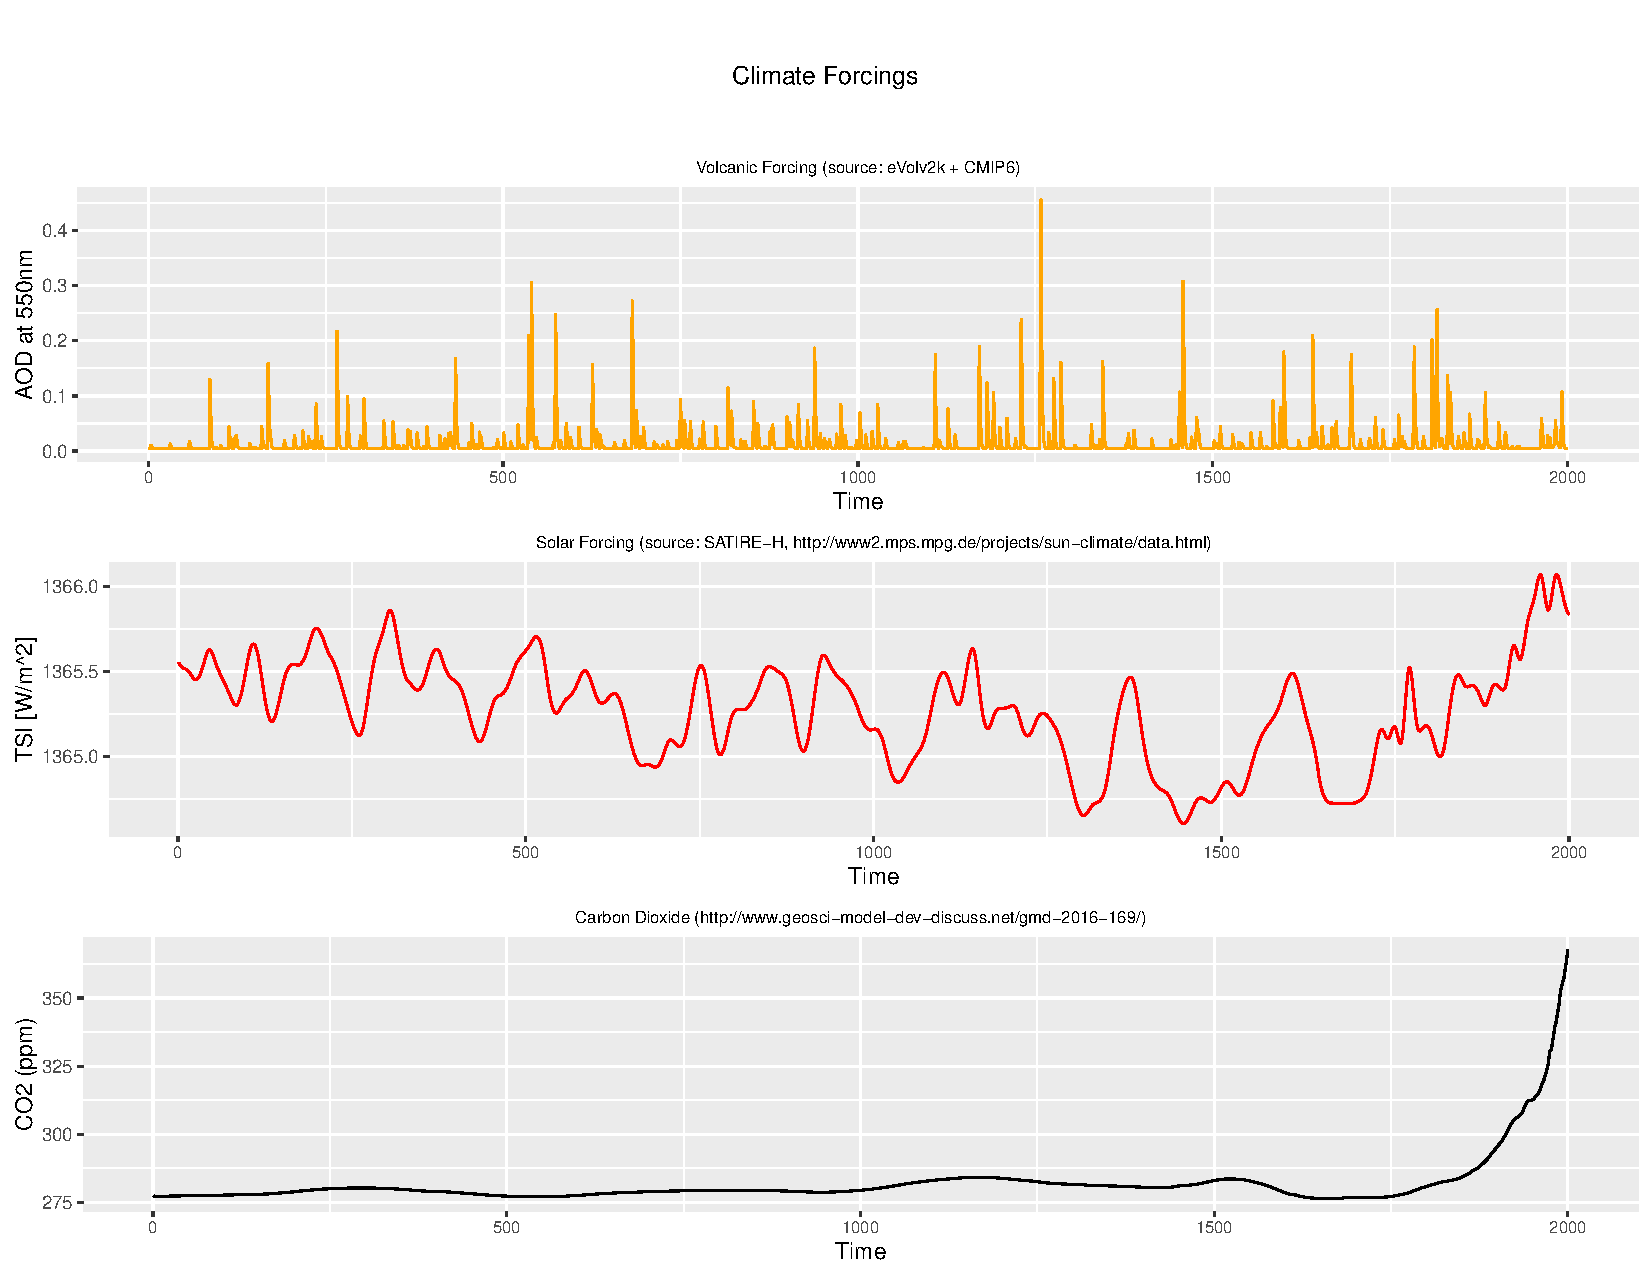
\includegraphics[scale=0.4]{forcings}
  \caption{Climate Forcings in the Common Era (1-2000 AD)}
  \label{fig:forcings}
\end{figure}

\begin{figure}[H]
  \centering
  \includegraphics[scale=0.4]{RecCE_S3}
  \caption{Paleoclimate Reconstruction in the Common Era (CE) with 95\%
    prediction bands. Scenario 3.}
  \label{fig:paleoCE3}
\end{figure}

\begin{figure}[H]
  \centering
  \includegraphics[scale=0.4]{Rec1900_S3}
  \caption{Paleoclimate Reconstruction 1900-2000 with 95\%
    prediction bands. Scenario 3.}
  \label{fig:paleo19003}
\end{figure}
\end{document}
